\chapter{Introduction}
\thispagestyle{empty}

The nucleus is a self-organized system. The complexity of the
nuclear many-body problem has made nuclear physics a field driven
by discoveries of outstanding phenomena. With access to secondary
exotic nuclear beams, the edges of the nuclear landscape itself
are being explored, {\em i.e.} the very limits of nuclear
existence. At these limits, the so-called neutron (proton) {\em
driplines}, additional neutrons(protons) literally drip out of the
nucleus. The exact locations of the boundaries are far from clear,
and their complete determination awaits a better quantitative
understanding of the nuclear system. Nuclei far from stability
allow us to amplify and isolate particular aspects of the nuclear
interaction and dynamics. Using what we learn from these nuclei we
can then return to the nuclei of the world around us and
understand them far better than ever before. Progress in nuclear
structure is made at the various levels where one attempts to
understand nuclear phenomena; (i) Experimental data and
phenomenology, (ii) `Local models' (effective models with few
emergent degrees of freedom),
 (iii) `Global nuclear models',
(iv) Ab initio NN-interaction based procedures, (v) QCD.
There is an overall effort to explain higher levels in terms of
lower ones, but a more reductionist ``deductive approach'' is
likely to have as precursor an approach which tries to isolate and
understand the characteristic degrees of freedom. 

\section{Halo Nuclei; Clusters and a Veil of extremely Dilute and
Extended Neutron Matter}


%\begin{wrapfigure}{r}[0pt]{5.5cm}
\begin{figure}[tb]
%\begin{center}
%\includegraphics[scale=0.33]{lisize.eps}
%\end{center}
\centerline{\psfig{figure=figures/lisize.eps,width=8cm}}
\vspace{3mm}
\caption{The matter size of $^{11}$Li is compared to
that of $^{48}$Ca and $^{208}$Pb \label{Size} }
%\end{wrapfigure}
\end{figure}

The granularity of a halo nucleus, say that of the cardinal case
of $^{11}$Li, is not trivial, see Fig.~\ref{Size}. The spatial
extension is huge, the rms matter radius of $^{11}$Li is as large
as that of $^{48}$Ca, and the radius of the halo neutrons is as large
as for the outermost neutrons in $^{208}$Pb. It is a true
challenge for theory to account for both extension and
granularity.

Light nuclei constitute so far the part of the nuclear landscape
where the neutron dripline has been reached.  Triggered by
Tanihata's discovery (1985) \cite{isao} of vastly spatially
extended nuclei ($^{6,8}$He; $^{11}$Li; $^{11}$Be) at the neutron
dripline, the initial idea of (binary) halos was suggested by B.
Jonson and P.G. Hansen \cite{Hansen}. Subsequent developments have
deepened and enriched the picture of halos as outstanding
structural dripline phenomena with extreme clusterization into an
ordinary core nucleus and veil of halo nucleons -- forming
exceptionally dilute neutron matter. The origin of the
stratification is purely quantum mechanical in nature, and only partly
understood, but a prerequisite is low angular momentum motion for
the halo particles and few-body dynamics such as in Borromean
nuclei\footnote{ The three Borromean rings, the heraldic symbol of
the Italian Borromeo family, are interlocked in such a way that if
any of them were removed, the other two would also fall apart. The
three interwined Borromean rings are now widely used as the logo
of the halo field.} characterized by pairwise constituents with no
bound states. In the limit of vanishing binding, extremely large
halos may occur.

In a remarkable paper in atomic physics in 1988 \cite{macek},
``Loosely bound states of three particles'', Zhen and Macek write;
``Although  there is no corresponding experimental data to confirm
these results at present, the theory is nevertheless of great
interest because it predicts some new physical properties of
three-body systems, among which the most remarkable one is the
existence of loosely bound states in such systems, even though the
interaction potential between the particles has no wells strong
enough to bind any two of the three particles separately. Because
of this, and since the three-body system is the simplest  model in
many-body problems, it seems desirable to use the three-body
system (instead of two-body) as the basic block of the many-body
system''.

The dream had already come true, three years earlier  --  but in
another field, at the neutron dripline when Isao Tanihata and his
team made their discoveries in 1985. In the following decade
$^6$He and $^{11}$Li became understood as realizations of exactly
the mechanisms Zhen and Macek were speaking about, and were in 1993
baptized Borromean halo nuclei \cite{zhuk}. At that time we were,
however, not aware of the Zhen/Macek paper.

The Borromean property is clearly exhibited by the hadronic
stability of various isotope chains, see Fig.~\ref{Map}. Thus,
while $^5$He is unbound $^6$He is bound, $^7$He is unbound but
$^8$He is again bound. A recent review \cite{jonson} looks at
all the dripline nuclei.

\begin{figure}[tb]
%\begin{center}
%\includegraphics[scale=0.4,angle=270]{segre.eps}
%\end{center}
\centerline{\psfig{figure=figures/segre.eps,width=8cm,angle=270}}
\vspace{3mm}
\caption{The nuclear chart exhibits the stability of
Borromean nuclei among different isotope chains \label{Map}}
\end{figure}

Pioneering activities usually employ some kind of scaffolding and
the
 discoveries are highlighted in terms of heuristic interpretations.
 These emphasize the new findings, and halo physics is no exception. The binary
 core-(point)dineutron picture of Hansen and Jonson for two-neutron halos
 (1987), originally just meant to illustrate how large extension and weak
 binding may be related, turned out to be an oversimplification.
 Since 1990, halo models have been developed where the N-N degree of freedom is
 no longer frozen, but chosen in accordance with the free NN interaction
 inspired by the dilute character of the halo. Thus focus has been shifted to
 features genuinely related to the intrinsic character of the halo, and of the
 interplay between halo degrees of freedom.

  The present picture of a `normal' nucleus veiled in a neutron halo,
 i.e. co-existence of normal and low density nuclear material, has emerged from
 a concerted effort between subsequent dedicated measurements and theory. How
 this stratification takes place still needs to be better understood, but
 nature seems to have provided a laboratory where `eigenproperties' of the
 low-density halo can be studied, subjected only to a mild influence from the
 intrinsic structure of the core object.
Few-body dynamics plays the crucial role in any adequate
description of halo properties, since for halo bound states most
of the wave function is concentrated in the classically forbidden
region. The chain of He isotopes with an alpha core has become
particularly  useful as set of benchmark systems.

In three-body models of halo nuclei such as $^6$He, Pauli blocking
is needed to remove components of the halo wave function that
would disappear under full antisymmetrization. This, and also
other aspects of the composite nature of the clusters make the
challenge somewhat different from that of three-nucleon systems.

\subsection{Enriching the Nuclear Paradigm}

Thomas Kuhn, in his famous book ``The Structure of Scientific
Revolutions'', claims that we are hypnotized by our paradigms.
Kuhn's conclusions are questioned by Steven Weinberg in a recent
article ``The Revolution That Didn't Happen'', in the New York
Review \cite{weinb}. In particular Weinberg argues that ``He
(Kuhn) was quite wrong in saying that it is no part of the work of
normal science to find new sorts of phenomena''. Here we side with
Weinberg. New  discoveries, also fundamental, do not as a rule
require overthrowing paradigms, they rather extend and modify a
ruling paradigm. What we are doing these days is to enrich and
widen the nuclear paradigm. The lessons we have learned during the
last decade or so by directing, with increasing success, our
nuclear studies toward extreme conditions are truly remarkable.

The recent theory advances have influenced dripline physics
conceptually, and also its methodology and logistics. Two-body
recipes have been replaced by appropriate 3-body (few-body)
theory. And most importantly: a theory framework with growing
predictive power is emerging.

The Hoyle resonance in $^{12}$C plays a crucial role in the
synthesis of the elements; ``It wouldn't be missed if it didn't
exist'' to paraphrase a statement by the Danish writer Piet Hein.
{\it It is the doorway to our Universe.} The processes leading to
this doorway {\it all proceed} from $^4$He {\it via Borromean
systems}: (i) in Red Giants via the triple $\alpha$-process; (ii)
in Supernovae via $^9 _4$Be$_5$ also Borromean; and (iii) a less
probable side-route to $^9$Be via $^6$He. Recall that neither
$(\alpha \alpha)$, $(\alpha n)$ nor $(n n)$ can form bound binary
systems, only resonances.

\section{Simplicity in Complexity}

It is customary in fields with a rich history to try to fit the
new findings within the ruling formalisms: in nuclear physics a
many-particle shell model type picture. The shell model has,
however, not turned out very suited for halo systems, and has to
be fundamentally modified for neutrons so close to the continuum
threshold. We will return to this. The concept of orbits in the
sense of relative motions with respect to the core, is on the
other hand still fruitful. Thus the recognition of the
instrumental role of low angular momentum "intruder" orbits (s and
p) has become essential to our understanding of exotic structure
formation and the melting of shell structures at the neutron
dripline. Borromean nuclei is most easily understood in a
three-body cluster formulation, using the Hyper Harmonic method,
which for bound states gives the leading physics in terms of only
a few wave function components \cite{zhuk}.

A dream dating back to the early years of nuclear physics is that
of starting from the free binary interactions, for reactions as
well as structure. The influence of the nuclear  medium has
complicated this approach. For loosely bound dripline nuclei this
question has renewed interest. The nature of the halo seems
sufficiently dilute to justify approaches where the starting point
is the free nucleon-nucleon t-matrix.

\subsection{Borromean Halos: Three-body Theory}

Fig.~\ref{figLi11} gives an impression of the average (r.m.s.)
geometrical separations in $^{11}$Li, indicating also the ranges
of the interactions between the constituents. The geometry of the
figure corresponds to three-body calculations, the gross structure
is however insensitive to finer details of the calculations. For
$^6$He the relative geometry is quite similar, the core radius is
now 1.5~fm. The abnormal size of the halo systems is obviously
related to the unusually small separation energies ($\sim$ 1 MeV or
less), and means that there is a large probability (often more
than 50\%) of the system being in classically forbidden
configurations. The situation is truly one of `residence in
forbidden regions' \cite{riisager94}.

\begin{figure}[tbph]
\begin{center}
\includegraphics[scale=0.5]{figures/lithium2.eps}
\end{center}
%\centerline{\epsfxsize=7cm\epsffile{lithium2.eps}} \vspace*{2mm}
\caption{The geometrical structure of $^{11}$Li and its core
$^9$Li
 with r.m.s radii $3.5\,$fm and $2.3\,$fm, exhibiting Borromean
 tunneling into classically forbidden regions.
 The ranges of the binary interactions are indicated.
 Distributing the 11 nucleons with a usual Fermi-type density
 distribution would give about 1/3 of normal nuclear density.}
\label{figLi11}
\end{figure}

The physical building blocks for describing such systems are, just
like for transfer reactions, appropriate overlap functions ${\cal
O}^A_C(x) = \langle \Psi_C(C) ~|~ \Psi_A(C,x) \rangle$ (where $x$
are the translationally invariant halo coordinates) between a
given state $A$ for the halo nucleus and a possible state $C$ for
the core. In a few-body model,
the overlap coincides with the few-body wave function.

The asymptotic behaviour of a one-neutron overlap between bound
states is simply $\exp(-\kappa^A_C r_{1C})$ where $r_{1C}$ is the
relative coordinate between the core and the valence neutron while
the decay constant  $\kappa^A_C = \sqrt{2\mu_{1C}S^A_C}/\hbar$ is
governed by the separation energy  between the two states being
connected.

The asymptotic behaviour becomes essentially more complicated
already for two halo neutrons. For Borromean nuclei \cite{zhuk},
however, it simplifies to  $\exp(-\kappa^A_C \rho)$ where $\rho$
is the hyperradius, expressed in $n$-$n$ and ($nn$)-$C$ relative
distances as
$$
\rho^2 = \frac{1}{2} r^2_{nn} + \frac{2C}{C+2} r^2_{(nn)C}
$$
while the decay constant now is $\kappa^A_C =
\sqrt{2MS^A_C}/\hbar$ and $S^A_C$   the two-neutron separation
energy, $M$ is the nucleon mass. There is also a quantum number
$K$, being the hypermoment quantum number associated with the
`angular'  $\alpha$ conjugate of the hyperradius $\rho$. This is
essentially a generalisation of the transformation to polar
coordinates in the 2-body case.

If an initial expansion of the three-body wave function on
hyperspherical harmonics (HH) is used \cite{zhuk}, the three-body
Schr\"{o}dinger equation simply becomes a set of coupled equations
for radial amplitude functions {\Large$\chi$}$_{K\gamma}(\rho)$ in
the hyperradius. The mathematical scheme bears a resemblance with
that of a particle in a strongly deformed field
$V_{K\gamma,K'\gamma'}(\rho)$:
\begin{eqnarray}
& &\Bigl( - \frac{\hbar^2}{2M} \Bigl[ \frac{d^2}{d\rho^2} -
\frac{(K+3/2)(K +5/2)}{\rho^2} \Bigr] + V_{K\gamma,K\gamma}(\rho)
- E
\Bigr) \mbox{\large $\chi$}_{K\gamma}(\rho)  \nonumber \\
& &~~~=   - \sum_{K'\gamma' \not= K\gamma} V_{K\gamma,
K'\gamma'}(\rho) \mbox{\large $\chi$}_{K'\gamma'}(\rho).
\label{hcc}
\end{eqnarray}
The coupling matrix elements are
\begin{equation}
V_{K'\gamma', K\gamma}(\rho) = \langle{\cal Y}_{K\gamma}(\Omega_5)
\mid \sum_{j\not=i\ =1}^{3} V_{ij}\mid {\cal Y}_{K'\gamma'}
(\Omega_5) \rangle
\end{equation}
 %
where $V_{ij}$ are the binary potentials and $\gamma = \{ l_x,
l_y, L, S \}$. Here $l_x$  and $l_y$ are relative angular momenta,
say $l_x=l_{nn}$, $l_y=l_{(nn)C}$ in the di-neutron set of Jacobi
($T$-)coordinates, while $\Omega_5$ contains the hyperangle
$\alpha$ in addition to the four spatial angles of a Jacobi set.
The hypermoment  $K=2n+l_x+l_y$ for some integer $n$ = 0, 1, 2 ...
 %
For bound states ($E<0$) each {\Large$\chi$}$_{K\gamma}(\rho)$ is
regular for $\rho \rightarrow 0$ and falls off exponentially as
$\exp(-\kappa_C^A \rho)$ for  $\rho \rightarrow \infty$.

For a Borromean system the above HH equations can easily be solved
for continuum states at positive energy $E>0$. The asymptotic
boundary condition is again a generalisation of binary scattering
to that of $3\rightarrow 3$ scattering and is given in the
hyperradius by $\chi_K^{K'}(\rho)\rightarrow
H^-_K(\rho)\delta_{KK'} -S_{KK'}H^+_K(\rho)$ for a
unit-amplitude boundary condition in channel $K'$.

Borromean systems have no binary binding. So why is the system
bound? Part of the explanation is related to the three-body HH
centrifugal barrier, the term in eq.(\ref{hcc})  which is
proportional to $ (K+3/2)(K+5/2)/\rho^2 $. Even if $K=0$, implying
that the total orbital angular momentum is zero, the three-body
centrifugal barrier does not vanish, contrary to the two-body
case. For sufficient binding between the bodies, this may provide
a barrier inside which quasi-bound motion may be established, giving
rise to three-body resonances in the continuum, even if there are
only $s$-wave virtual states in the binary subsystems.
Furthermore, as Efimov \cite{efim90} first pointed out, the
attraction in $\rho$ contains components of asymptotic behaviour
$\rho^{-3}$ for the diagonal terms.

\subsection{Two-neutron Borromean Ground States}

The test-bench three-body Borromean halo nucleus has been $^6$He.
The ground-state properties of  $^6$He  are quite well determined
by the known $\alpha - n$ and $n-n$ pairwise potentials, and a
variety of few-body calculations have been performed for the
ground state wave function, and these are largely in agreement
with each other. They support a picture in which the valence
neutrons have a 90\% probability of being in a $(0p_{3/2})^2$
configuration, with the $n-n$ attraction increasing the $S=0$
component of the wave function from an uncorrelated $67\%$ to a
correlated 89\%. The structure of the $0^+$ ground state of
$^6$He, with its spatial density dominated by a ``di-neutron'' and
a ``cigar'' peak, is shown in fig.~\ref{he6rr}, and has  been
reproduced by a number of few-body procedures. `Pure three-body'
models using pairwise interactions underbind $^6$He by around 0.5
MeV. This is almost certainly due to the neglect of the $t+t$
degree of freedom.

%\begin{figure}
\begin{wrapfigure}{l}[0pt]{6cm}
\begin{center}
\includegraphics[scale=0.3]{figures/reahe6fc.drrr2b.eps}
\end{center}
%\centerline{\epsfxsize=12cm\epsffile{reahe6fc.drrr2b.eps}}
\caption{The joint radial probability of the halo neutrons in
    $^6$He, averaged over all angles.  The rightmost peak
    has the two neutrons closest together.
} \label{he6rr}
\end{wrapfigure}
%\end{figure}

The ground-state properties of  $^{11}$Li are not so well
determined, since the available information on the binary
neutron-$^9$Li(core) channel is not sufficiently unambiguous and
non-contradictory. It is now generally agreed, based on a variety of observables,
that in a two-neutron halo system such as
$^{11}$Li, the intruder $(1s_{1/2})^2$ two-particle configurations
can be mixed by the $nn$ interaction with the $(0p_{1/2})^2$
configuration, so the ground state will be roughly an equal
superposition of these two arrangements for $^{11}$Li. The weights
and wave functions are given by the solution of the three-body
problem. We predicted \cite{Thompson94} that the presence of a
low-lying $s$ virtual (antibound) state in the $n+^9$Li system,
when included in three-body calculations, would have a pronounced
effect on the structure of the $^{11}$Li halo.

Low-energy two-neutron transfer reactions with Borromean nuclei
have been shown to be an effective instrument for studying both
the structure of such nuclei and the dynamics of nuclear reactions
where they take part. A four-body model has been developed to
describe such two-nucleon transfer processes within DWBA, and also
extended to coupled reaction channels. Using a realistic 3-body
bound state wave function of $^6$He, the role of its separate
components has been thoroughly studied. In particular, it was
found that the ``di-neutron'' configuration of the $^6$He nucleus
gives the dominant contribution to the two-neutron transfer cross
sections, measured at FLNR, Dubna, \cite{zag2}. The possibilities
of using multi-neutron transfer reactions for studying the
structure of other radioactive nuclei, such as $^8$He, have now
become part of the schedule at leading international laboratories.

\section{Exciting a Halo to the Borromean Continuum}

Dripline physics, involving nuclei with only one or a few weakly
bound states, is physics of threshold phenomena where structure and
reaction theory merge. Recently the theoretical few-body approach
has been successfully extended to also encompass three-body
continuum structure, response functions and reactions involving
Borromean systems. Borromean continua, for which the three-body
threshold is the lowest-lying, are intriguing. Here the continuum
pairing, and also the different decay channels via low-lying
binary resonant states, can change shell-model expectations
drastically. An example is the $^6$He nucleus with only one
experimentally confirmed narrow ($2^+$) resonance below the $t+t$
threshold at 13 MeV. The nature of experimentally observed
strength concentration at 1--3 MeV (from three-body threshold) in
$^6$He, and at 1 MeV in $^{11}$Li, is being clarified. The
strength may contain three-body resonances, or a new kind of collective motion
-- an induced giant dipole moment due to oscillations of the inert
core against the halo neutrons -- that does not correspond to a
pole in the S-matrix.

The intrinsic properties of Borromean continua are directly
revealed in $3\rightarrow3$ scattering, which however is almost
impossible to perform experimentally, but could be significant in
neutron stars and supernovi. In ordinary binary reactions the
continuum is usually explored via responses that induce
transitions from the ground state to the continuum. A reliable way
to study halo continuum properties is one-step transitions in
nuclear reactions. A microscopic four-body reaction theory has
recently been developed \cite{ershov1}, a rather comprehensive task
because of the intertwining of the ground state and continuum
structures, influenced by reaction mechanisms.

\begin{figure}[tbh]
\vspace*{-0.2cm}
\begin{center}
\begin{tabular}{c}
\includegraphics[scale=0.31]{figures/2+nnj=2-2.eps} %      here enter the name
\includegraphics[scale=0.31]{figures/2+cnj=2-2.eps}      \\
\includegraphics[scale=0.31]{figures/1mnntot2.eps} %      here enter the name
\includegraphics[scale=0.31]{figures/1mcntot2.eps}
\end{tabular}
\end{center}
\vspace*{-0.2cm}
\caption{  Energy correlation plot for $2^+$ and $1^-$states in
$^6$He :
          with
         $1^-$ FSI (lower row) and intrinsic correlations for $2^+$
          (upper row). Left: in cluster {\bf T} basis, right: in
          `quasishell'-model {\bf Y} basis. }
\label{CorrPlot}
\end{figure}

In the vicinity of a `true' three-body resonance the $3\rightarrow
3$ scattering asymptotic amplitude has the analytical property
\begin{equation}   \label {merk3}
 A(E_{\kappa}) \sim
      {c \over {E_{\kappa} - (E_{0}-i \Gamma_0/2)}}
\end{equation}
where $E_{\kappa}$ is the excitation energy calculated from the
three-body threshold. $E_{0}$ and $\Gamma_0$ are the position and
width of the resonance, while $c$ depends on spatial and momentum
angles in hyperspherical coordinates \cite{zhuk}. This coincides
in the two-body case with the resonant structure of the wave
function in the interior region, a property we have also observed
(but not proved) for the Borromean three-body case :
 \begin{equation}\label{intnorm1}
 \psi(\rho; E_{\kappa}) \sim
      C(E_{\kappa}) ~~ \psi^R (\rho)
\end{equation}
 with
\begin{equation}
|C(E_{\kappa})|^2 = {const \over (E_{\kappa} - E_{0})^2 +
\Gamma_0^2/4}
\end{equation}
where $ \psi^R(\rho)$ is the energy-independent form of the
internal part of the scattering wave function. Using this
resonance representation for the wave function in transition
matrix elements, a factorised expression for the exclusive cross
section for three-body fragmentation can be obtained. After
integration over the directions of momenta $\vec{k}_x, \vec{k}_y$
between the fragments, the double differential cross-section
becomes proportional to :
\begin{equation}\frac{d^{2} \sigma} {d\varepsilon_{x_{i}} d\varepsilon_{y_{i}}}
\sim \sqrt{\varepsilon_{x_{i}} \varepsilon_{y_{i}}}\
|C(E_{\kappa})|^2 \sim {\sqrt{\varepsilon_{x_i} \varepsilon_{y_i}}
\over (\varepsilon_{x_{i}} + \varepsilon_{y_{i}} - E_{0})^2 +
\Gamma_0^2/4} \nonumber \\
\end{equation}
%
where $\sqrt{\varepsilon_{x_i} \varepsilon_{y_i}}$ is the phase
volume accessible to fragments in three-body decay.


Thus it is
clear that a correlation plot of $d^{2} \sigma /d\varepsilon_{x_i}
d\varepsilon_{y_i}$ should have maxima along a ridge which is the
straight line $E_0 = \varepsilon_{x_i} + \varepsilon_{y_i}$ with
sections in a contour plot of elliptical type with width $\sim
\Gamma_0$. Halo neutrons and core can be combined in two different
ways ($T$ and $Y$) into binary Jacobian subsystems. One ($T$) is
when the $x$-coordinate corresponds to the $n-n$ subsystem while
$y$ refers to $C-(nn)$. In the second case ($Y$) the $x, y$ denote
$C-n$ and $(Cn)-n$, respectively. The excitation energy
$E_{\kappa}$ and the phase volume $\sqrt{\varepsilon_{x}
\varepsilon_{y}}$ are invariant for any binary Jacobian partitions. Then
the ridge pattern of the energy correlation plot should be similar
in $T$ and $Y$ partitions in the case of a true three-body
resonance, and modified if not. This is a {\it decisive} tool for
identification of a true three-body resonance directly from
experimental data, in addition to calculated phase shifts.


%\begin{figure}[th]
\begin{wrapfigure}{l}[0pt]{6.5cm}
%\vspace*{-1.5cm}
\begin{center}
\includegraphics[scale=0.4]{figures/He6PbC2.eps}
\end{center}
%\vspace*{-2cm}
\caption{Spectrum of $^6$He in collision with
(a) $^{12}$C  and (b) $^{208}$Pb at energy E/A 240 MeV. Dotted, thin
solid and dashed lines are the monopole, dipole and quadrupole
excitations, respectively.
See \protect\cite{ershov1} for further detail.
\label{He6PbC} }
\end{wrapfigure}
%\end{figure}

The most extensive and reliable analysis has been carried out for
$^6$He where as a check point the known $2^+_1$ resonance is
reproduced. The calculations give $1^-$ strength concentrations at
lower energies (soft modes) in the proximity of the three-body
threshold and predict new $2^+$, $1^+$ (and possibly $0^+$)
resonances at slightly higher energies in $^6$He.
Fig.~\ref{CorrPlot} shows how a correlation plot can be used to
prove that while $2^+_1$ is a `true' three-body resonance, the
much debated $1^-$ dipole strength is not!



This correlated microscopic continuum structure has been used to
gain new insight in halo fragmentation in diffractive breakup.
Thus the crucial role of the low-lying three-body resonances and
soft modes in determining distribution characteristics (width and
shape) has been demonstrated. A surprising memory of the low-lying
continuum structure prevails even in inclusive observables.
Fig.~\ref{He6PbC} shows GSI data and calculations \cite{ershov1} for
$^6$He break-up to the halo continuum.

\section{Ab initio Calculations of Halos}

The most ambitious of these `reductionist' attempts are Green's
Function Monte Carlo (GFMC) calculations \cite{pudl}, extending
previous variational Monte Carlo (VMC). According to the authors
these are the first microscopic calculations that directly
produce nuclear  shell structure from realistic interactions that
fit NN scattering data. Another line of approach are the
large-basis no-core shell-model (NCSM) calculations of Barrett's
group \cite{bruce1,bruce2,bruce3,bruce4}, where the shell model is combined with
microscopic effective interactions derived from modern
nucleon-nucleon potentials. Substantial progress has been made in
recent years, but a three-body (Illinois) interaction has to be
supplemented to make the  GFMC able to bind loosely bound halo
systems like $^6$He and $^8$He.

The size of the GFMC (and NCSM) calculations, regrettably, grows
beyond what is manageable even before $^{11}$Li is reached. The
practitioners have, however, already had success with their
pioneering attempts. Thus the GFMC calculations for A=6 do produce
an alpha-like core object, and two alpha-particles for $^8$Be,
both promising features.

To check the information content in GFMC type wave functions, a
joint venture with few-body modeling is needed to explore critical
observables and to improve the asymptotic behavior of GFMC. Work
to this end will require the best available computer support.

\section{Expansions on a Berggren Basis}

In nuclear physics, expansion of complex objects on an unperturbed
single (two) particle basis, generated by a suitable potential,
has been common practice. In the traditional shell model the
harmonic oscillator basis has served as a paradigmatic tool for
describing bound nuclei, providing a reasonable description for
the more deeply bound single particle orbitals. As one approaches
the nuclear driplines the binding reduces, and in the Borromean
limit the core-n interaction is unable to uphold bound motion.
Thus there will be no bound state part in the usual completeness
relation, or \emph{resolution of unity}, proven by Newton in
Ref.~\cite{newton},
\begin{equation}
\label{eq:unity1} {\bf 1} = \sum_{nl}
\vert\psi_{nl}\rangle\langle\psi_{nl}\vert + \sum_{l}{1\over
2}\int_{-\infty}^{\infty} dk
k^2\vert\psi_{l}(k)\rangle\langle\psi_{l}(k)\vert.
\end{equation}

The exploration of the nuclear driplines has now pushed the
traditional many body methods to their limits of applicability,
and coupling to the binary continuum  plays a vital
role. A modification of the shell model has become known as the
\emph{Gamow shell model}, see Refs.~\cite{witek1,betan}, or the {\it
Berggren expansion}, where bound, resonant, antibound and continuum
states are treated on equal footing, and has been under
development for
the last few years. As alluded to earlier, we had to include
antibound (virtual) $s$ motion in our three-body calculation of
$^{11}$Li to understand the physics findings of this remarkable
system. Recently the role of antibound states in the Gamow shell
model description of this system has also been discussed \cite{betan}.

The study of two-body resonant structures has a long history in
theoretical physics. There exists a variety of methods described
in for example textbooks such as \cite{newton}. Among the more
popular methods one finds the complex scaling method (CSM) and the
method based on analytic continuation in the coupling constant
(ACCC).

Recently we have considered an approach formulated for integral
equations in momentum space.  The method is based on deforming the
contour integrals in momentum space, and known as the contour
deformation or distortion method (CDM). It has been shown
previously that a \emph{contour rotation} in momentum space is
equivalent to a rotation of the corresponding differential
equation in coordinate space. The coordinate space analog is often
referred to as the \emph{dilation group transformation}, or
\emph{complex scaling}.

Complex scaling in coordinate space has for a long time been used
extensively in atomic and molecular physics, see
Ref.~\cite{nimrod}. During the last decade it has also been applied
in nuclear physics, as interest in loosely bound nuclear halo
systems has grown, see for example Refs.~\cite{csoto}.

There are several advantages in considering the contour
deformation method in momentum space. First, most realistic
potentials derived from field theoretical considerations are given
explicitly in momentum space. Secondly, the boundary conditions
are automatically built into the integral equations. Moreover, the
Gamow states in momentum space are non-oscillating and rapidly
decreasing, even for Gamow states with large widths far from the
real energy axis, as opposed to the complex scaled coordinate
space counterpart. These states are represented by strongly
oscillating and exponentially decaying functions.

\begin{figure}[hbtp]
\begin{center}
\includegraphics[scale=0.4]{figures/gen_cont.eps}
\end{center}
\caption{Contour $ C_{R+T}^{+} = L_{1} + L_{2} + L_{3} $ is given
by the solid line, while the contour $C_{R+T}^{-} $ is given by
the dashed line. The contour $C_{R+T} = C_{R+T}^{+}+C_{R+T}^{-}$
is clearly \emph{inversion symmetric}. The two body spectrum which
is exposed by this contour is marked by filled circles $ \bullet $
and the excluded spectrum by open circles $\circ $. The full
spectrum includes bound states (B), anti-bound (A), decay (D) and
capture (C) resonant states.  } \label{fig:contour2}
\end{figure}

A revitalising of the contour deformation method in momentum space
has therefore taken place. CDM is a method which allows for
accurate and stable solutions of binary bound, anti-bound,
capture, and decay states. We consider a generalized type of
contour, allowing for an analytic continuation in the third
quadrant of the complex $k$-plane. Antibound - and capture states
near the scattering threshold may then be calculated at a
specified accuracy.  This choice of contour can be regarded as a
special case of the \emph{Berggren class} of contours
\cite{berggren}. Berggren studied various completeness relations
derived by analytic continuation of the Newton completeness
relation to the complex plane. The Berggren completeness includes
discrete summation over resonant as well as bound states.
Figure~\ref{fig:contour2} gives an example of a Berggren type
contour which also includes antibound states. To solve a many-body
problem by expansions on a Berggren basis is no straightforward
task. An important lesson so far for Borromean halos is that the
continuum states on the complex contour give vital contributions,
in addition to those from physical resonances and antibound
states.

\section{Conclusions}

After a decade of work, essential physics of Borromean bound
states in two-nucleon halo nuclei is now understood in terms of a
three-body cluster model formulation. The stratification itself
has, however, to be understood at a deeper nucleonic level and
encouraging developments to this end, such as within the Green's
function Monte Carlo method, have been reported in recent years.
These methods are also tools to understand multi-neutron halos,
such as for $^8$He, where a cluster formulation involves the
challenges of the five-body problem. Loosely bound multi-neutron
matter within halos provides a fascinating laboratory for
low-density research. With few bound states close to multifragment
break-up threshold, investigations of the physics of halo continua
represent another direction of research in rapid development,
involving also need for a better understanding of few-body
reaction theory. We have given the status of the art for Borromean
two-neutron halos.

\section{Overall motivation and aims}
\label{sec:motivation}

\section{Exploring exotic structures by complex scaling techniques}
\label{sec:exploring_exotic}

\section{Challenges for the newly developed Gamow Shell Model}
\label{sec:challenges}


